\documentclass[]{ceurart}


\sloppy

\usepackage{graphicx} 
\usepackage{amsmath}
\usepackage{amssymb}
\usepackage{array}
\usepackage{mdwmath}
\usepackage{mdwtab}
\usepackage{eqparbox}
\usepackage{url}
\usepackage{graphicx}
\usepackage{tabularx,booktabs}
\usepackage{diagbox}
\newcolumntype{C}{>{\centering\arraybackslash}X}
\setlength{\extrarowheight}{1pt}
\hyphenation{op-tical net-works semi-conduc-tor}
\usepackage{algorithm,algorithmic}
\usepackage{pifont}
\newcommand{\cmark}{\ding{51}}
\newcommand{\xmark}{\ding{55}}

\newcommand{\revision}[1]{\textcolor{blue}{#1}}

\usepackage{adjustbox}
\usepackage{listings}
\lstset{breaklines=true}

\begin{document}


\copyrightyear{2023}
\copyrightclause{Copyright for this paper by its authors.
  Use permitted under Creative Commons License Attribution 4.0
  International (CC BY 4.0).}


\conference{Second International Workshop on Linked Data-driven Resilience Research (D2R2'23) co-located with ESWC 2023, May 28th, 2023, Hersonissos, Greece}


\title{A News Recommendation System for
Environmental Risk Management}

\tnotemark[1]

\author[1]{Hamed Aboutorab}[%
orcid=0000-0002-9285-9917,
email=h.aboutorab@unsw.edu.au]
\cormark[1]
\address[1]{University of New South Wales, Canberra, Australia }

\author[2]{Ran Yu}[%
orcid=0000-0002-1619-3164,
email=ran.yu@uni-bonn.de]


\author[2]{Alishiba Dsouza}[%
orcid=0000-0001-5884-6234,
email=dsouza@cs.uni-bonn.de]
\address[2]{Data Science \& Intelligent Systems Group (DSIS), University of Bonn, Bonn, Germany}


\author[3]{Morteza Saberi}[%
orcid=0000-0002-5168-2078,
email=morteza.saberi@uts.edu.au]
\address[3]{University of Technology Sydney, Sydney, Australia}

\author[1]{Omar Khadeer Hussain}[%
orcid=0000-0002-5738-6560,
email=o.hussain@adfa.edu.au]


\cortext[1]{Corresponding author.}

\begin{abstract}
Environmental risk events, such as flooding, can disrupt freight routes and cause business losses. It is therefore crucial to proactively identify and manage these risks. When identifying environmental risks, it is essential to examine the impact of these events on freight routes. In this paper, we extract knowledge about environmental risk events from the knowledge graph and build a machine-learning model to identify freight routes potentially affected by floods. We propose a news recommendation system, namely the News Recommender for Environmental Risk Identification \& Analysis (NR-ERIA), to recommend news related to a location of interest that has the risk of being affected by environmental risk events to support the risk management.
We conducted experiments on real-world datasets and achieved an accuracy of 0.908 in proactively detecting disruptions, which is 196\% higher than the baseline approach, demonstrating the effectiveness of our proposed system.

\end{abstract}

\begin{keywords}
  Risk Identification \sep
  Environmental Risk \sep
  News Recommender System 
\end{keywords}

\maketitle
\section{Introduction}\label{1}
Accurately identifying the environmental risks that can cause disruptions to freight routes is an important task that can benefit various downstream applications, such as road safety management and the prevention of business losses due to transport disruptions. 
News is one of the major sources for web users to get information on environmental risks. 
Recently, researchers have been investigating news recommenders for effective risk management. For example, Aboutorab et al. \cite{aboutorab2021reinforcement} developed a news recommender to identify the possibility of risk events affecting a company's operations from news articles.

 While these models are more efficient and effective than their predecessors, there are open challenges that need to be addressed, such as the large amount of irrelevant information that they may present to the user. This occurs for a number of reasons, one of which is that the capture of geographic location based on keywords in news articles is insufficient for the system to accurately identify the geographic area where the risk event may have an impact. 

In this paper, we present our preliminary work in building a news recommender system to address the above-mentioned issue and minimize the amount of irrelevant information presented to the user. 
To recommend the relevant news, the system not only determines if an environmental risk event is going to occur but also identifies the geographical area that is affected by the risk event.
This requires, firstly, a comprehensive knowledge of the characteristics of different types of risk events and, secondly, the examination of news articles to determine the precise areas that may be affected. To the best of our knowledge, these challenges have not been addressed by existing news recommender systems \cite{raza2022news}. In this work, we extract knowledge about risk events, such as floods, from one of the largest openly available cross-domain knowledge graphs (KG) DBpedia\footnote{\url{https://www.dbpedia.org/}} \cite{articledbpedia}, and use it to guide the feature extraction in our framework. The extracted features are further used to determine if a location will be affected by a risk event. 
Based on the disruption detection result and user relevance feedback, we build the news recommendation system NR-ERIA.
We evaluate the performance of the proposed model by conducting experiments on a real-world dataset containing 1000 historical road closures due to environmental risk events. NR-ERIA achieved better performance in terms of accuracy, precision, and F1 score compared to the baseline model for identifying news of affected locations, demonstrating the effectiveness of our proposed model. 


\section{Related Work}\label{sec:related_works}
In this section, we review the research on environmental risk identification. Environmental risk can be defined as the destructive human activities on the planet \cite{jones2001environmental} or the impact of natural disasters on business operations \cite{coburn2013taxonomy}, the latter being the focus of our work. This type of risk has been studied extensively, for example, Powell et al. \cite{powell2016system} used system knowledge to study the impact of flooding on power stations. Ravankhah et al. \cite{ravankhah2017multi} developed a model to identify the impact of seismic events on the world's cultural heritage sites.

In recent years, environmental risk identification models have been significantly improved through the integration of AI techniques. For example, Aboutorab et al. \cite{aboutorab2021reinforcement} proposed an RL-based recommender system that proactively identifies disruptions. More than 60 researchers have developed vision-based approaches for flood detection and management \cite{munawar2021review}. For example, Pally et al. \cite{pally2022application} have integrated image processing and convolutional neural networks (CNN) to identify the depth, severity, and extent of flooding. The studies are not limited to flood analysis. Boillot et al. \cite{boillot2021deep} used deep learning to study seismic facies. Liu et al. \cite{liu2019local} have developed a method to identify severe storms using measurements from a geostationary weather satellite. 

However, one of the shortcomings of these methods is that they do not take into account the precise location of the disruption. Another shortcoming is that they focus on only one type of environmental risk event. In this paper, we develop a framework for Environmental Risk Identification and Analysis (NR-ERIA) that assesses environmental risk events (i.e. flood, earthquake, storm) and identifies the exact affected area.

\section{NR-ERIA Approach}\label{3}

This section explains the framework of NR-ERIA, which consists of three modules: 1) the disruption identification module extracts important factors of environmental risks that cause disruptions and identifies disruptions accordingly; 2) the news retrieval \& analysis module retrieves news articles that are relevant for disruptions caused by environmental risk events; 3) the news recommendation module brings the relevant news about critical disruption events to the user's attention. Figure \ref{RL-ERIA} illustrates the conceptual framework of NR-ERIA.

\begin{figure}[h]
  \centering
  
  \includegraphics[page=2,trim=0cm 4.5cm 3cm 0.5cm, width=0.8\textwidth]{photo/overview.pdf}
  \caption{NR-ERIA conceptual framework}\label{RL-ERIA}
  \vspace{-0.2in}
\end{figure}

\subsection{Identifying Disruptions Caused by Environmental Risks} \label{sec:radius}

In this module, given a specific type of environmental risk, the aim is to predict whether a location of interest will be affected by a risk event of the given type. 
We consider the area to be a circle centered on the location of interest $a$ with radius $R$. 

The risk factors of a location of interest are represented by a feature vector. The features are extracted from DBpedia\footnote{\url{https://www.dbpedia.org}}, a knowledge graph that contains rich structured information of entities, including the common type of environmental risks. To extract the features, we first obtain the textual description of the given type of environmental risk (e.g. flood) from the property of interest (e.g. \textit{dbo:abstract}), then apply the cause-effect detection tool based on token classification with BERT \footnote{\url{https://huggingface.co/noahjadallah/cause-effect-detection}} to determine the main causes of the given environmental risk and use them as features. 
For modeling the radius $R$, we apply the One-Class Classification Support Vector Machine (OCC SVM)\footnote{\url{https://scikit-learn.org/stable/modules/generated/sklearn.svm.OneClassSVM.html}} \cite{DBLP:journals/neco/ScholkopfPSSW01} as it can learn the boundaries from data samples without additional human supervision. 

As a use case, we study the environmental risk type \textit{flooding}. Using the feature extraction approach introduced above, we extract four features: \emph{precipitation rate} (millimeter) and \emph{distance from rivers} (kilometer), \emph{lakes} (kilometer), and \emph{oceans} (kilometer). 
For model training, we obtain the historical data of road closures due to flooding from the Australian government website \footnote{https://datahub.freightaustralia.gov.au} at different locations and compute the corresponding feature vectors for each location, and use the average numerical values of features for the OCC SVM to learn the radius $R$ that will be used for future prediction of whether a location of interest falls into the \textit{affected} class. 
The OCC SVM first forms the \emph{affected} class as a hypersphere by the center of $a$ and the radius $R$ around the data and tries to minimize the volume to contain training objects $x_i$ ($i=1,...,n$) as 

\begin{equation}\label{OCCnormal}
    \min_{R, a}R^2
\end{equation}

subject to

\begin{equation}\label{OCCconstraints}
    \parallel{x_i - a}\parallel{^2}\leq R^2, i=1,...,n
\end{equation}

Equation \ref{OCCnormal} is modified to Equation \ref{OCCnormal1} to provide a soft margin of $\xi_i\geq0$ to decrease the restriction and tolerate outliers in the training set.

\begin{equation}\label{OCCnormal1}
    \min_{R, a, \xi}R^2 + C\sum_{i=1}^n\xi_i
\end{equation}

subject to

\begin{equation}\label{OCCconstraints1}
    \parallel{x_i - a}\parallel{^2}\leq R^2 + \xi_i, i=1,...,n
\end{equation}

where $C$ is a parameter used to adjust the balance between volume and errors. At the end of this phase, NR-ERIA is able to predict whether the location of interest will be affected by the given type of environmental risk, i.e. flooding.

\subsection {News Retrieval \& Analysis} \label{sec:news_retrieval}

This module monitors current news articles and analyses them against the \emph{affected} class created in the previous module. More specifically, each news article is parsed to extract locations. We apply the named entity recognition provided by python library \textit{spaCy}\footnote{\url{https://spacy.io/}} for the location extraction. For each location $l$, we use the model described in \ref{sec:radius} to check if it is in the \emph{affected} class. A news article is identified as important to be shown to the user if it is relevant to a \textit{affected} location.

This module also takes into account user feedback on relevance. A database named \emph{archived} is created in this module to record how interesting the recommended news is to the user. This is done by labeling the news article as \emph{relevant} and \emph{irrelevant} based on user feedback in the next module (RL-based news recommender). News articles shortlisted based on the module introduced in Section \ref{sec:radius} are further vectorized using the Term Frequency-Inverse Document Frequency (TF-IDF) \cite{sammut2011encyclopedia}. 
These vectors are then used to train an SVM model to classify the news articles into \textit{relevant} and \textit{irrelevant} classes. To do this, we use the $C$ support vector classification presented in LIBSVM \cite{chang2011libsvm}. 

With respect to the flood case study, we extract locations from the news, compute the values of the features such as Precipitation rate, and distance from rivers, lakes, and oceans for the locations, and classify whether the location is in the \textit{affected} area.
For the \textit{relevant} and \textit{irrelevant} classes, we simulate user relevance feedback based on the historical dataset by annotating the news articles relevant to the location of road closures as \textit{relevant} and the rest as \textit{irrelevant}. In real-world applications, the model is able to adapt to the user's perceived relevance. 

\subsection {News Recommender}

In this module, a news article that belongs to both the \emph{affected} class (mentions a location that is highly likely to be at risk of disruption) and the \emph{relevant} category (is highly likely to be considered relevant by the user) is presented to the user via email. The concept of Explainable AI (XAI) \cite{gunning2019xai} is also taken into account to explain to the user why this news article is being displayed. The likely impact on the locations of interest is presented alongside the news article for better understanding. Figure \ref{RL-ERIA email} shows an email sent by NR-ERIA. NR-ERIA then receives feedback in the form of a \cmark or \xmark~ from the user. The news articles shown to the user are labeled \emph{relevant} if the feedback is positive (\cmark), otherwise (\xmark) labeled \emph{irrelevant} and stored in the \emph{archive} database.

\begin{figure}[hbt!]
  \begin{center}
  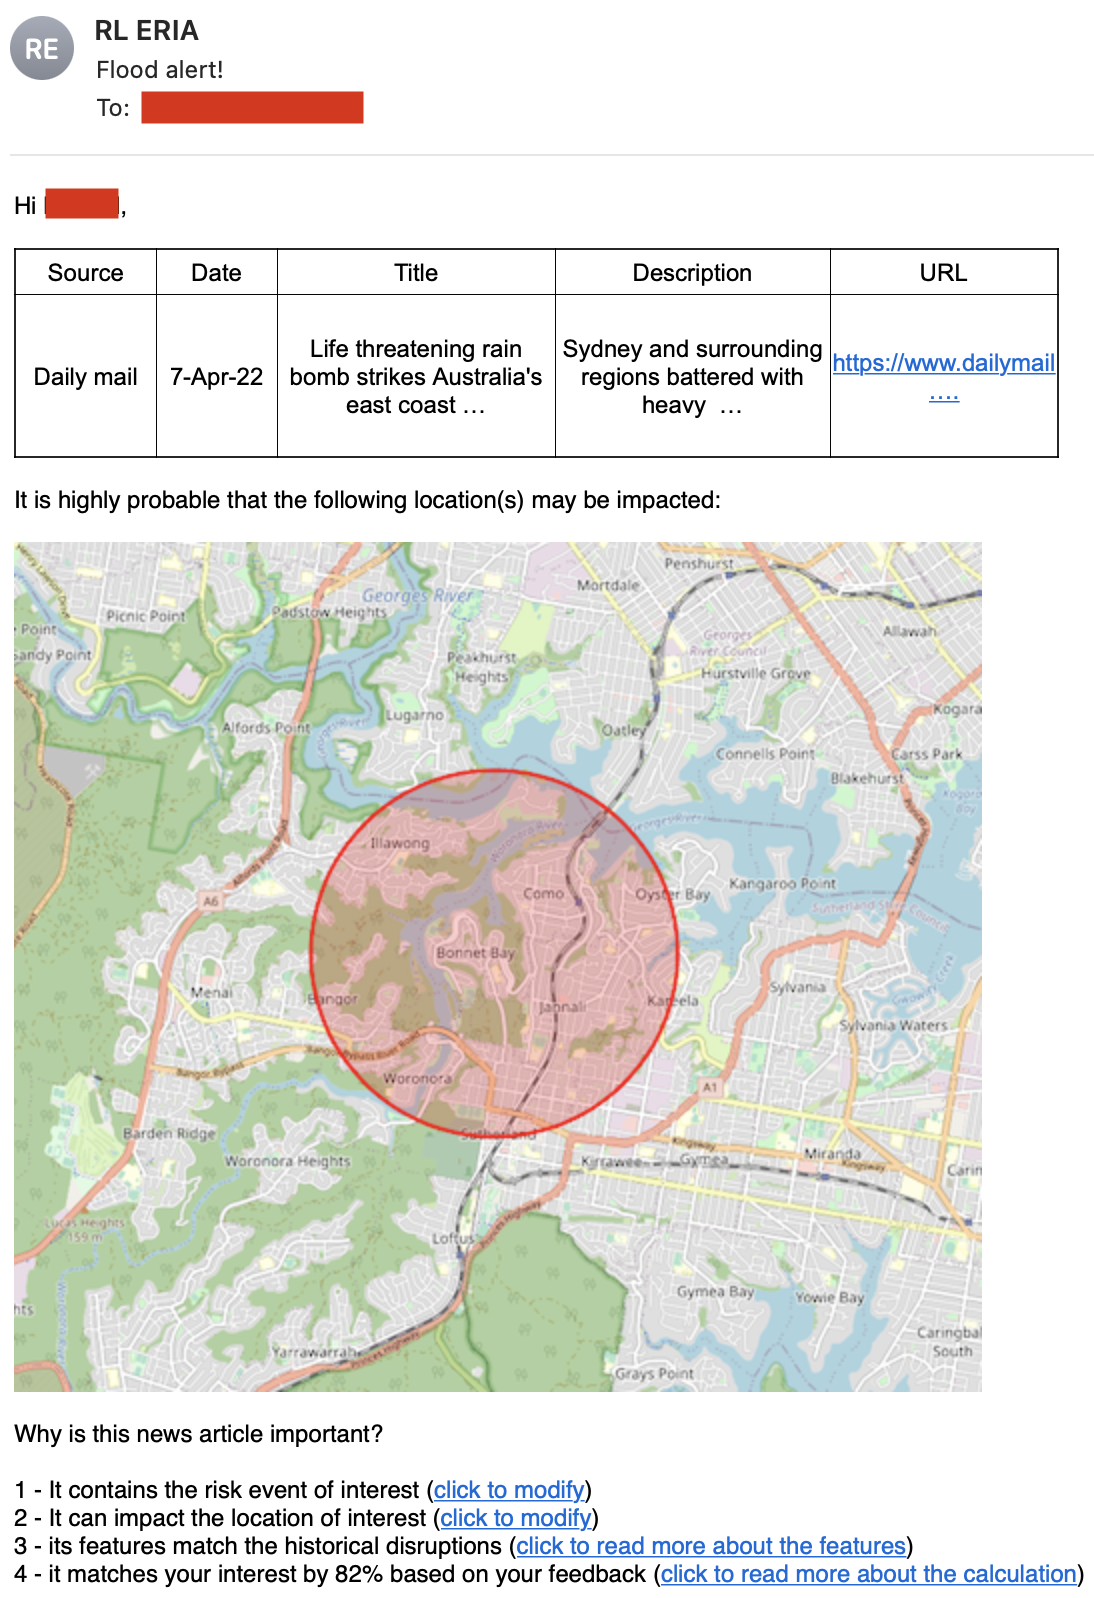
\includegraphics[width=4.2in]{photo/email.png}\\
  \caption{An email sent by NR-ERIA }\label{RL-ERIA email}
  \end{center}
  \vspace{-0.2in}
\end{figure}

\section{Performance Analysis of NR-ERIA}

In this section, we evaluate the performance of NR-ERIA. We consider the environmental risk of flooding in our experiment. We perform the evaluation in three steps. First, we evaluate the NR-ERIA algorithm in terms of its ability to identify the risk of a location being affected by an environmental risk based on its geographic features. 
Second, we compare the performance of NR-ERIA with the existing approach for proactive risk identification (RL-PRI) model proposed by Aboutorab et al. \cite{aboutorab2021reinforcement}, in terms of disruption risk identification. Finally, the ability of NR-ERIA to identify which news articles are most likely to be of interest to the user is analyzed.

\subsection{Assessment of NR-ERIA's Ability in Identifying Disruptions Caused by Environmental Risks}

In this evaluation, we use the dataset of 1000 historical road closures due to flooding provided by the Australian government \footnote{https://datahub.freightaustralia.gov.au} as our case study. As mentioned in the Data Preparation module, by using the DBpedia dataset and cause-effect detection, we identify precipitation rate and distance from rivers, lakes, and oceans as the important features and obtain their values for all these locations and dates. To do this, we first obtain the average weekly precipitation rate for each location and date by using Meteostat \footnote{https://meteostat.net/en/}. Secondly, the lakes and coastlines polygons and the rivers line strings are extracted from the Natural Earth website \footnote{\url{https://www.naturalearthdata.com}} and the Euclidean distance from each point to any point on the line strings is calculated. Table \ref{tab:RL-ERIA e1} shows one row of this dataset.

\begin{table}[h]

\caption{1 row of \emph{normal} dataset for 1000 road closures due to flood}
\label{tab:RL-ERIA e1}
  \centering
  \adjustbox{max width=\textwidth}{
  \begin{tabular}{p{2cm}|p{2.5cm}|p{3cm}|p{1.5cm}p{1.5cm}p{1.1cm}|p{2cm}}
    \toprule
     Date & Location & Coordinate & \multicolumn{3}{c|}{Distance from (km)} & Precipitation (mm)\\
     & & & River & Lake & Ocean & \\
    \midrule
  12/10/20 & Armstrongs Rd & (-38.568, 145.982) & 227.322 & 228.008 & 62.471 & 6.428\\
\midrule
  \end{tabular}}
\end{table}


We then use this data to train our model and create the \textit{affected} class. For the evaluation, we use the accuracy, i.e. the percentage of correct predictions of whether a location will be \textit{affected} by flooding. 
We use 10-fold cross-validation, i.e. we randomly divide this dataset of 1000 road closures into 10 parts, for each run 900 samples are used for training and 100 for testing the model performance. 
NR-ERIA achieves an accuracy of 0.92 in identifying the location of disruptions caused by flooding in this case study.



\subsection{Comparison of NR-ERIA and RL-PRI in the Identification of News Articles Covering Disruptions Caused by Environmental Risk Events}

We compare the performance of NR-ERIA with the RL-PRI model proposed by Aboutorab et al. \cite{aboutorab2021reinforcement}. This experiment evaluates the performance of the two models in identifying the risk of disruption from news articles. In the case of the flood as the risk event of interest, we consider the news articles reporting information related to road closures caused by flood to be of importance to the user. 
We use the same dataset as in baseline work \cite{aboutorab2021reinforcement} for disruption detection, which contains 348 news articles, and 93 of them are annotated as containing information about flood-related road closures. 

We apply location extraction, as introduced in section \ref{sec:news_retrieval}, to the news articles to obtain the locations they contain, and then perform location risk identification, as introduced in section \ref{sec:radius}, to decide whether the news mentions a location that will be \textit{affected} by the flood. 
We then calculate the number of true positives (TP), false positives (FP), false negatives (FN), and true negatives (TN) based on the results of NR-ERIA and RL-PRI. The definitions and results of TP, FP, FN, and TN are given in the list below and in Table \ref{tab:RL-ERIA e4} respectively.

\begin{itemize}
    \item TP: Road closure due to flooding and presented by the model.
    \item FP: No road closures and presented by the model.
    \item FN: Road closure due to flooding and not presented by the model.
    \item TN: No road closures and not presented by the model.
\end{itemize}

\begin{table}[h]
\caption{TPs, FPs, FNs, and TNs of NR-ERIA and RL-PRI.}
\label{tab:RL-ERIA e4}
  \centering
  \adjustbox{max width=0.5\textwidth}{
  \begin{tabular}{>{\centering}p{0.15\textwidth}>{\centering}p{0.15\textwidth}>{\centering}p{0.2\textwidth}}
    \toprule
    Category & RL-PRI & NR-ERIA \\
    \midrule
 $TP$ & 87 & 78 \\
 $FP$ & 235 & 17 \\
 $FN$ & 6 & 15 \\
 $TN$ & 20 & 238 
 \\ \bottomrule
  \end{tabular}}
\end{table}

Finally, we calculate the accuracy, precision, and recall on the positive class and the F1 score for these two models \cite{ting2017encyclopedia} in correctly presenting news articles containing locations with disruption risk due to flooding. Table \ref{tab:RL-ERIA e5} shows the results of the comparison between RL-PRI and NR-ERIA. The results show that NR-ERIA outperforms RL-PRI in terms of accuracy and F1 score. The reason for this is that NR-ERIA considers more environmental risk-specific factors (e.g. distance to rivers) that are important for the identification of disruptions compared to RL-PRI. 
Regarding the trade-off between precision and recall, NR-ERIA achieves an increase in precision of 0.55 and a decrease in recall of 0.1. In the context of news recommendation, considering that important events are usually reported by multiple channels, a slight decrease in recall would not have a major impact on the utility of the recommender.

\begin{table}[h]
\caption{$a$, $p$, $r$, and $F1$ scores of the environmental risk identification by RL-PRI and NR-ERIA}
\label{tab:RL-ERIA e5}
  \centering
  \begin{tabular}{ccc}
    \toprule
    \textbf{Metric} &\textbf{ RL-PRI} & \textbf{NR-ERIA} \\
    \midrule
  $accuracy$ & 0.31 & \textbf{0.91}\\
 $precision$ & 0.27 & \textbf{0.82}\\
 $recall$ & \textbf{0.94} & 0.84\\
 $F1$ & 0.42 & \textbf{0.83}\\
    \bottomrule
  \end{tabular}
\end{table}

\subsection{Evaluation of NR-ERIA's Capability in Recommending News Articles That Match Users' Interest}
In this evaluation, we analyze NR-ERIA in terms of its ability to decide whether a news article is of interest to the user by classifying it into the \textit{relevant} or \textit{irrelevant} class (Section \ref{sec:news_retrieval}). In this evaluation, for each road closure, we collect news articles that mention the region of the closed road in the period of 10 days before and after the road closure. We use the location of the road closure as a keyword and query in Google News (e.g., flood Abergowrie Road Queensland), and filter the search results with time constraints. We simulate user feedback by considering the news articles that mention at least one of the road closures in locations of interest to the user (in this case, overlapping with regions the user has business operations) as relevant and the rest as irrelevant. We annotate 500 news articles using this strategy and test the performance of our model using 10-fold cross-validation. In each round of experiments, 450 news articles are used to train the model and 50 are used to test its performance. We repeat this process 9 more times. Table \ref{tab:RL-ERIA e3} shows the performance metrics \textit{accuracy}, \textit{precision} and \textit{recall} of the positive (i.e. relevant) class and the F1 score of NR-ERIA.


\begin{table}[h]
\caption{NR-ERIA's performance on recommending relevant news articles.}
\label{tab:RL-ERIA e3}
  \centering
  \begin{tabular}{p{2cm}p{1.5cm}p{1.5cm}p{1.5cm}p{1.5cm}}
    \toprule
     & \textit{accuracy} & \textit{precision} & \textit{recall} &\textit{ F1}\\
    \midrule
    \textbf{RE-ERIA} & 0.71 & 0.77 & 0.71 & 0.74\\
    \bottomrule
  \end{tabular}
\end{table}

The results show that NR-ERIA achieves a good overall performance with an accuracy of 0.71 and an F1 score of 0.74. The balance between precision and recall guarantees that users can obtain satisfactory results of interest and, in the meantime, have the opportunity to explore new topics.

\section{Conclusion}\label{5}

In this paper, we have proposed NR-ERIA, a framework for recommending news articles containing information relevant to potential disruptions caused by environmental risk events. NR-ERIA is capable of proactively identifying disruption risks from news sources and presenting them to interested users. Experimental results show that NR-ERIA can reduce the amount of irrelevant information presented compared to the baseline approach RL-PRI, thus providing more accurate recommendations. In addition, NR-ERIA demonstrates good performance in adapting to relevant feedback from users. In future work, we will focus on building more advanced models, such as models that can make use of multimodal information (e.g. images and videos) in news. Although we have conducted our preliminary experiments on the case study of flooding, this framework can be applied to risk types such as forest fires and financial risks provided that the corresponding features are extracted from knowledge bases. In future work, we plan to investigate more types of environmental risks and to involve real users in our analysis.


%%
%% The acknowledgments section is defined using the "acknowledgments" environment
%% (and NOT an unnumbered section). This ensures the proper
%% identification of the section in the article metadata, and the
%% consistent spelling of the heading.
\begin{acknowledgments}
  %This work was partly funded by the DFG -- German Research Foundation under (``WorldKG'', 424985896), and the DAAD Programme for Project-Related Personal Exchange (PPP) from 2022 with Australia under the project ``KOALA''.

This work was partially funded by the DFG, German Research Foundation (``WorldKG'', 424985896), and DAAD, Germany (``KOALA'', 57600865).

\end{acknowledgments}

 \bibliography{cas-refs}




\end{document}

